\documentclass[11pt,a4paper]{article}

\usepackage[utf8]{inputenc}
\usepackage[T1]{fontenc}
\usepackage[spanish,es-nodecimaldot]{babel}
\usepackage{lmodern}
\usepackage{microtype}
\usepackage[a4paper,margin=2.5cm]{geometry}
\usepackage{graphicx}
\usepackage{booktabs}
\usepackage{tabularx}
\usepackage{array}
\usepackage{amsmath}
\usepackage{amssymb}
\usepackage{float}
\usepackage{xcolor}
\usepackage{enumitem}
\usepackage{hyperref}

\definecolor{linkblue}{HTML}{1D4ED8}
\hypersetup{
    colorlinks=true,
    linkcolor=linkblue,
    citecolor=linkblue,
    urlcolor=linkblue,
    pdftitle={Informe módulo taller: charruaLLM},
    pdfsubject={Desarrollo y evaluación de un modelo de lenguaje para noticias uruguayas}
}

\setlist{itemsep=0.25em, topsep=0.4em}
\setlength{\parindent}{0pt}
\setlength{\parskip}{0.65em}
\renewcommand{\arraystretch}{1.15}
\emergencystretch=2em

\newcommand{\charrua}{\texttt{charruaLLM}}
\newcommand{\spanishmodel}{\texttt{spanishLLM}}
\newcommand{\code}[1]{\texttt{#1}}

\title{\textbf{Informe módulo taller}\\[0.5em]
\large Desarrollo y evaluación de \charrua:\\
un modelo de lenguaje autoregresivo entrenado con noticias uruguayas}
\author{Juan Pablo Conde, Bruno Turcatti}
\date{\today}

\begin{document}

\maketitle
\thispagestyle{empty}

\begin{abstract}
Este trabajo presenta el desarrollo y la evaluación de \charrua, un modelo de
lenguaje Transformer autoregresivo de 17,1 millones de parámetros entrenado con
UY22, el corpus de noticias uruguayas presentado junto con ROUBERTa. Para
estudiar el efecto de la especialización de dominio se entrenó un segundo
modelo, \spanishmodel, con la misma arquitectura y un corpus general en español.
Además, se construyó un conjunto de evaluación de 834 ejemplos a partir de
afirmaciones de QuUANTO, derivadas originalmente de QuALES. Los modelos se
compararon mediante exact matching de la palabra final y negative
log-likelihood (NLL) de sus tokens. \charrua{} obtuvo 26,62\,\% de exact
matching, frente a 4,68\,\% de \spanishmodel, y una NLL media por palabra de
4,1396, frente a 22,8143. Los resultados muestran una ventaja clara del modelo
especializado, en línea con los hallazgos de ROUBERTa, aunque deben
interpretarse considerando las diferencias entre tokenizadores, capitalización
y posible solapamiento de dominios.
\end{abstract}

\clearpage
\tableofcontents
\clearpage


\section{Breves antecedentes}

Los modelos de lenguaje modernos estiman la probabilidad de una secuencia de
texto a partir de sus componentes. En un modelo autoregresivo, la probabilidad
de una secuencia de tokens $t_1,\ldots,t_n$ se factoriza como

\begin{equation}
    P(t_1,\ldots,t_n)
    = \prod_{i=1}^{n} P(t_i \mid t_1,\ldots,t_{i-1}).
\end{equation}

Esta formulación permite entrenar un modelo con texto sin etiquetar mediante
una tarea simple: predecir el token siguiente. La arquitectura Transformer,
introducida por Vaswani et al.~\cite{vaswani2017}, sustituyó la recurrencia de
arquitecturas anteriores por mecanismos de atención. Esto permitió modelar
dependencias entre posiciones de una secuencia y paralelizar mejor el
entrenamiento.

A partir del Transformer surgieron dos grandes familias de modelos de lenguaje:
los modelos de tipo encoder, como BERT y RoBERTa, y los modelos autoregresivos
decoder-only, como GPT y GPT-2. El modelo desarrollado en este trabajo pertenece
a la segunda familia. Su objetivo no es clasificar texto ni responder preguntas
mediante fine-tuning, sino aprender una distribución sobre el texto y generar
continuaciones mediante predicción del token siguiente.


\subsection{RoBERTa}

RoBERTa, cuyo nombre significa \emph{A Robustly Optimized BERT Pretraining
Approach}, es una revisión de la receta de entrenamiento de BERT presentada por
Liu et al.~\cite{liu2019}. El trabajo mostró que parte de las mejoras atribuidas
a nuevas arquitecturas podía obtenerse entrenando BERT durante más tiempo, con
lotes mayores y más datos. También eliminó el objetivo de \emph{Next Sentence
Prediction}, utilizó secuencias más largas y aplicó enmascaramiento dinámico.

RoBERTa es un modelo encoder y se entrena con \emph{masked language modeling}:
recibe información a ambos lados de una posición enmascarada. Por ello no es la
arquitectura usada directamente en \charrua, que genera texto de izquierda a
derecha. Sin embargo, es un antecedente relevante por dos motivos. Primero,
muestra que los datos y el régimen de entrenamiento pueden importar tanto como
los cambios arquitectónicos. Segundo, el sistema ganador de la tarea QuALES
2022 empleó un modelo RoBERTa multilingüe preentrenado y ajustado para preguntas
y respuestas~\cite{rosa2022}. Esto aporta un punto de referencia para el origen
del dataset que luego adaptamos a nuestra evaluación de completado de palabras.


\subsection{ROUBERTa: antecedente directo sobre el corpus UY22}

El antecedente más cercano a este trabajo es ROUBERTa, presentado por Filevich
et al.~\cite{filevich2024} en \emph{A Language Model Trained on Uruguayan
Spanish News Text}. El nombre combina RoBERTa con ROU, sigla de República
Oriental del Uruguay. El artículo introdujo UY22, un corpus específico de
prensa uruguaya, y entrenó desde cero variantes \textit{cased} y \textit{uncased} de un modelo
RoBERTa sobre su versión limpia.

UY22 reúne aproximadamente 900.000 artículos, 400 millones de palabras y más
de 6~GiB de texto sin comprimir, con noticias publicadas desde comienzos de la
década del 2000 hasta diciembre de 2022. Sus cuatro fuentes son El Observador,
El País, Montevideo Portal y La Diaria. El proceso de limpieza incluyó la
eliminación de HTML y espacios duplicados, normalización de caracteres,
eliminación de emojis, reemplazo de enlaces y descarte de artículos con menos
de 16 palabras.

ROUBERTa utiliza una arquitectura encoder de tipo RoBERTa-base, un tokenizer
BPE de 30.000 tokens y dynamic masked language modeling con una probabilidad de
enmascaramiento del 15\,\%. Fue entrenado durante 30 días y unos seis millones
de pasos en una NVIDIA P100 de 12~GiB. El entrenamiento comenzó con una
longitud máxima de 384 tokens y luego continuó con longitud 128 y batch size 32
para ajustarse a la memoria disponible. La versión pública tiene un orden de
magnitud de 100 millones de parámetros
\footnote{Ficha del modelo: \url{https://huggingface.co/pln-udelar/ROUBERTa-base-uy22-cased}.},
por lo que sigue siendo considerablemente mayor que los 17,1 millones de
parámetros de \charrua.

El artículo evaluó ROUBERTa en análisis de sentimiento, Question Answering y
predicción de palabras enmascaradas. La variante cased alcanzó 75,0\,\% de
accuracy en sentimiento y, después de fine-tuning sobre QuALES, obtuvo 28,1 de
Exact Match y 32,3 de F1. En siete textos periodísticos recientes y no vistos,
predijo correctamente 982 de 2.368 palabras enmascaradas, un 42\,\% de top-1,
frente al 27\,\% obtenido tanto por BETO como por XLM-RoBERTa.

Dos ablaciones del artículo son especialmente relevantes para nuestro
experimento. Primero, un RoBERTa entrenado con 4~GiB de UY22 alcanzó 68,6\,\%
en sentimiento, frente a 65,0\,\% de otro modelo entrenado con 20~GiB del corpus
general usado por BETO. Segundo, la variante cased alcanzó 75,0\,\%, frente a
68,6\,\% de la variante uncased. Estos resultados respaldan tanto la hipótesis
de especialización de dominio como la importancia de la capitalización que
observamos al comparar \charrua{} con \spanishmodel.

ROUBERTa y \charrua{} comparten el corpus de origen y la motivación de crear
modelos uruguayos utilizables con recursos limitados, pero resuelven objetivos
distintos. ROUBERTa es bidireccional: al completar una máscara puede utilizar
el texto ubicado a ambos lados de la palabra. \charrua{} es causal y solo puede
usar el contexto anterior. Por ese motivo, el 42\,\% de masked-word prediction
de ROUBERTa y el 26,62\,\% de exact matching de nuestro modelo no deben
interpretarse como una comparación directa de calidad.

\begin{table}[H]
    \centering
    \small
    \caption{Comparación conceptual entre ROUBERTa y \charrua.}
    \label{tab:ROUBERTa-charrua}
    \begin{tabularx}{\textwidth}{>{\bfseries}l X X}
        \toprule
        Aspecto & ROUBERTa & \charrua \\
        \midrule
        Corpus de origen & UY22 & UY22, versión procesada local \\
        Arquitectura & Transformer encoder, RoBERTa & Transformer decoder-only \\
        Objetivo & Masked language modeling & Predicción causal del token siguiente \\
        Contexto disponible & Izquierda y derecha de la máscara & Solo tokens anteriores \\
        Vocabulario & BPE, 30.000 tokens & Byte-Level BPE, 16.384 tokens \\
        Parámetros & Aproximadamente 0,1B & 17.114.880 \\
        Pasos reportados & Aproximadamente 6 millones & 960.000 \\
        \bottomrule
    \end{tabularx}
\end{table}


\subsection{GPT-2}

GPT-2 fue presentado por Radford et al.~\cite{radford2019} en \emph{Language
Models are Unsupervised Multitask Learners}. Es un Transformer decoder-only
entrenado con un objetivo causal: predecir cada token a partir de los tokens
anteriores. El trabajo mostró que, al aumentar la escala y la diversidad de los
datos, un mismo modelo autoregresivo podía adquirir capacidades útiles para
diferentes tareas sin modificar sus parámetros para cada una de ellas.

\charrua{} sigue esta idea central a una escala mucho menor y orientada al
español uruguayo. Al igual que GPT-2, utiliza atención causal, bloques
Transformer decoder-only, embeddings posicionales aprendidos y generación
autoregresiva. La diferencia principal está en la escala: el GPT-2 más grande
tenía 1.500 millones de parámetros, mientras que cada modelo de este trabajo
tiene 17.114.880 parámetros. Nuestro objetivo fue construir un modelo que
pudiera entrenarse con recursos académicos accesibles y estudiar el efecto del
dominio de los datos, no reproducir la escala de GPT-2.


\subsection{Chinchilla y elección de la cantidad de parámetros}

Hoffmann et al.~\cite{hoffmann2022}, en \emph{Training Compute-Optimal Large
Language Models}, estudiaron cómo distribuir un presupuesto de cómputo entre la
cantidad de parámetros del modelo y la cantidad de tokens de entrenamiento. El
resultado principal fue que ambos factores deben crecer de forma aproximadamente
pareja. El trabajo mostró que varios modelos grandes estaban subentrenados:
tenían demasiados parámetros para la cantidad de datos que habían procesado.
Como regla práctica derivada del estudio suele mencionarse un orden de magnitud
de aproximadamente 20 tokens de entrenamiento por parámetro, aunque no debe
interpretarse como una constante universal, especialmente fuera de las escalas
analizadas en el artículo.

Cada modelo de este proyecto tiene 17.114.880 parámetros. El corpus uruguayo
contiene 523.695.440 tokens en train, equivalentes a 30,60 tokens únicos de
train por parámetro. El corpus general en español contiene 735.225.214 tokens
en train, equivalentes a 42,96 tokens por parámetro. Estos cocientes muestran
que ambos corpus poseen suficiente volumen para el tamaño elegido.

No obstante, durante 960.000 pasos, con batches de 32 secuencias de 512 tokens,
cada entrenamiento presenta aproximadamente 15.728.640.000 posiciones de token
al modelo. Esto implica múltiples recorridos estadísticos sobre el corpus: unas
30 veces el tamaño del train uruguayo y unas 21 veces el del train general. Por
lo tanto, el experimento no debe describirse como una reproducción estricta del
óptimo de Chinchilla. La decisión práctica fue mantener un modelo pequeño y
entrenarlo extensamente. Con un presupuesto fijo de cómputo, el trabajo de
Chinchilla sugiere que también sería pertinente experimentar con un modelo de
mayor tamaño y menos repeticiones de los datos.


\subsection{Tokenización BPE}

Los dos modelos utilizan tokenizadores Byte-Level BPE independientes, con un
vocabulario de 16.384 tokens y el token especial
\texttt{<|endoftext|>}. BPE representa palabras frecuentes mediante uno o pocos
tokens y descompone palabras poco frecuentes en unidades menores
\cite{sennrich2016}. Esto evita depender de un vocabulario cerrado de palabras
completas y permite representar nombres propios, variaciones morfológicas y
caracteres acentuados.

La elección de tokenizadores independientes permite adaptar el vocabulario a
cada corpus, pero introduce una precaución al comparar métricas por token. Una
misma palabra puede tener diferente cantidad de tokens en cada modelo. En la
evaluación realizada, las 834 palabras objetivo produjeron 1.467 tokens con el
tokenizer de \charrua{} y 2.553 con el de \spanishmodel.


\section{Descripción del trabajo}

El objetivo fue construir un modelo de lenguaje base para noticias uruguayas en
español y medir si la especialización de dominio le permite anticipar mejor la
última palabra de afirmaciones relacionadas con noticias uruguayas. Para que la
comparación no dependiera únicamente del tamaño o de la arquitectura, también
se entrenó un segundo modelo con exactamente la misma configuración, pero con
un corpus amplio y heterogéneo en español.

El flujo de trabajo fue el siguiente:

\begin{enumerate}
    \item  Obtención y preparación del corpus  de noticias uruguayas UY22.
    \item Entrenamiento de un tokenizer Byte-Level BPE específico.
    \item Conversión del corpus a secuencias de identificadores de tokens.
    \item Separación por documentos en train, validation y test.
    \item Entrenamiento de \charrua{} mediante predicción del token siguiente.
    \item Preparación de un corpus general en español y entrenamiento de
          \spanishmodel.
    \item Creación de un dataset de evaluación, QuUANTO, con afirmaciones derivadas
    de pares pregunta-respuesta en QuALES.
    \item Evaluación mediante exact matching y negative log-likelihood (NLL).
    \item Almacenamiento de las predicciones y métricas en archivos CSV.
\end{enumerate}


\subsection{Arquitectura del modelo y cantidad de parámetros}

Ambos modelos comparten la arquitectura resumida en la
Tabla~\ref{tab:arquitectura}.

\begin{table}[H]
    \centering
    \caption{Configuración arquitectónica de los dos modelos.}
    \label{tab:arquitectura}
    \begin{tabularx}{0.82\textwidth}{>{\bfseries}l X}
        \toprule
        Componente & Configuración \\
        \midrule
        Tipo & Transformer autoregresivo decoder-only \\
        Capas Transformer & 6 \\
        Cabezas de atención & 6 por capa \\
        Dimensión del embedding & 384 \\
        Dimensión interna del MLP & 1.536 \\
        Contexto máximo & 512 tokens \\
        Vocabulario & 16.384 tokens \\
        Posiciones & Embeddings aprendidos \\
        Activación & GELU \\
        Normalización & Pre-norm con LayerNorm \\
        Atención & Scaled dot-product attention causal \\
        Dropout & 0,0 \\
        Capa de salida & Pesos compartidos con el embedding de tokens \\
        \bottomrule
    \end{tabularx}
\end{table}

Cada bloque utiliza conexiones residuales en los subbloques de atención y MLP.
La distribución exacta de parámetros se muestra en la
Tabla~\ref{tab:parametros}.

\begin{table}[H]
    \centering
    \caption{Distribución de parámetros del modelo.}
    \label{tab:parametros}
    \begin{tabular}{lr}
        \toprule
        Componente & Parámetros \\
        \midrule
        Embedding de tokens & 6.291.456 \\
        Embedding de posiciones & 196.608 \\
        Seis bloques Transformer & 10.626.048 \\
        LayerNorm final & 768 \\
        \midrule
        \textbf{Total} & \textbf{17.114.880} \\
        \bottomrule
    \end{tabular}
\end{table}

El peso compartido entre el embedding y la salida evita agregar otra matriz de
$16.384 \times 384$ parámetros. Todos los parámetros son entrenables.

La configuración de entrenamiento fue la misma para los dos modelos:

\begin{itemize}
    \item Optimizador AdamW, con $\beta_1=0{,}9$ y $\beta_2=0{,}95$.
    \item Learning rate máximo de $3\times10^{-4}$ y mínimo de
          $3\times10^{-5}$.
    \item Warmup de 200 pasos y decaimiento cosenoidal.
    \item Batch size de 32 y gradient accumulation igual a 1.
    \item Gradient clipping de 1,0 y weight decay de 0,1.
    \item 960.000 pasos de entrenamiento.
    \item Evaluación cada 250 pasos sobre 50 batches.
    \item Semilla de entrenamiento 1337.
    \item Cross-entropy para la predicción causal del token siguiente.
\end{itemize}


\subsection{Datos utilizados y procedencia}

\subsubsection{Corpus de \charrua}

El corpus utilizado pertenece a UY22, el mismo recurso presentado en el trabajo
de ROUBERTa~\cite{filevich2024}. El corpus original comprende El Observador, El
País, Montevideo Portal y La Diaria. La distribución publicada por sus autores
se muestra en la Tabla~\ref{tab:uy22}.

\begin{table}[H]
    \centering
    \caption{Composición del corpus UY22 reportada por Filevich et al.}
    \label{tab:uy22}
    \begin{tabular}{lrrr}
        \toprule
        Medio & Artículos & Palabras & Participación \\
        \midrule
        El Observador & 314.821 & 150.007.925 & 37\,\% \\
        El País & 147.004 & 92.605.424 & 23\,\% \\
        Montevideo Portal & 433.244 & 145.422.666 & 36\,\% \\
        La Diaria & 20.000 & 14.079.916 & 4\,\% \\
        \midrule
        \textbf{Total} & \textbf{915.069} & \textbf{402.115.931} & \textbf{100\,\%} \\
        \bottomrule
    \end{tabular}
\end{table}

La metadata del entrenamiento reproducido en este repositorio registra tres
archivos procesados, correspondientes a El Observador, El País y Montevideo
Portal:

\begin{itemize}
    \item \code{eo22-unified-splitted.txt};
    \item \code{ep22-unified-splitted.txt};
    \item \code{mp22-unified-splitted.txt}.
\end{itemize}

Las líneas no vacías se agruparon como documentos y los documentos se
separaron de forma reproducible con semilla 42. La partición resultante se
muestra en la Tabla~\ref{tab:datos}.

En consecuencia, el origen de los datos es UY22, pero la versión procesada que
figura en el checkpoint local contiene tres de sus cuatro medios y no registra
un archivo de La Diaria. La diferencia entre las aproximadamente 402 millones
de palabras informadas en el artículo y los 523,7 millones de tokens de nuestro
train se debe, además, a que una palabra puede convertirse en varios tokens BPE.

\begin{table}[H]
    \centering
    \caption{Particiones de los corpus utilizados.}
    \label{tab:datos}
    \begin{tabular}{llrr}
        \toprule
        Modelo & Split & Documentos & Tokens \\
        \midrule
        \charrua & Train & 884.682 & 523.695.440 \\
        \charrua & Validation & 4.468 & 2.658.412 \\
        \charrua & Test & 4.468 & 2.707.620 \\
        \midrule
        \spanishmodel & Train & 250.929 & 735.225.214 \\
        \spanishmodel & Validation & 1.263 & 712.293 \\
        \spanishmodel & Test & 1.304 & 808.811 \\
        \bottomrule
    \end{tabular}
\end{table}

Se reservó 0,5\,\% de los documentos para validation y 0,5\,\% para test. El
token \texttt{<|endoftext|>} se agregó al final de cada documento.

\subsubsection{Corpus de \spanishmodel}

Para construir un control de español general se emplearon muestras
preprocesadas y convertidas a minúsculas de 15 corpus que corresponden a la
composición de Large Spanish Corpus~\cite{canete}: DGT, DOGC, ECB, EMEA,
EUBookShop, Europarl, GlobalVoices, JRC-Acquis, News Commentary 11,
OpenSubtitles 2018, ParaCrawl, TED, UN, Spanish Wikis y MultiUN. Muchos de estos
recursos provienen de la colección OPUS~\cite{opus} y cubren dominios muy
distintos: legislación, documentos institucionales, medicina, noticias,
subtítulos, Wikipedia y transcripciones.

El train se dividió en 270.579 chunks y el material de origen ocupaba
3,0 GiB. Debido a su tamaño, se preparó mediante streaming,
asignación determinista de documentos a cada split y tokenización en chunks
acotados, sin cargar el corpus completo en memoria.


\subsection{Creación del nuevo dataset de evaluación}

Para evaluar el modelo se empleó QuUANTO, acrónimo de \emph{QuALES-derived
Uruguay Assertions for Neural Training Objectives}. Es un dataset de afirmaciones
declarativas en español derivadas de pares de pregunta-respuesta de QuALES. QuALES
fue una tarea de \emph{Question Answering} extractivo organizada en IberLEF 2022 y
basada principalmente en noticias uruguayas sobre la pandemia de COVID-19 y temas
relacionados~\cite{rosa2022}. Las afirmaciones para la evaluación se tomaron del
archivo \code{QuUANTO\_unified\_final.json} y del repositorio que documenta su
construcción~\cite{quanto}.

La construcción de QuUANTO combinó generación automática y revisión humana. En
primer lugar, un modelo de lenguaje convirtió cada par de pregunta y respuesta en
una afirmación autocontenida y marcó si su contenido dependía de un momento
específico. Luego se conservaron las afirmaciones no sensibles al tiempo y se
intentaron reescribir las restantes para expresar una formulación atemporal.
También se aplicaron filtrado de contenido relacionado principalmente con COVID-19
y correcciones del orden de la información. Finalmente, las afirmaciones fueron
sometidas a revisión humana. Este proceso
mejora la coherencia y la fidelidad respecto de la fuente, pero no equivale a una
verificación independiente de los hechos: el dataset hereda el sesgo temático y
periodístico de las noticias de QuALES.

Para convertir las afirmaciones en una tarea de completado se tomó la última
palabra de cada oración como objetivo y el resto como entrada. Por ejemplo:

\begin{quote}
\begin{tabular}{@{}ll@{}}
    \textbf{Afirmación:} & El Pereira Rossell es un hospital. \\
    \textbf{Entrada:} & El Pereira Rossell es un \\
    \textbf{Objetivo:} & hospital
\end{tabular}
\end{quote}

Se eliminó el punto final de la palabra objetivo y se mantuvo un espacio al
principio de \code{goal} para conservar correctamente el límite de palabra al
usar tokenizers Byte-Level. El resultado se guardó en
\code{final\_dataset.csv}, que contiene 834 ejemplos. Aunque cada afirmación
conserva el split original de QuALES como dato de procedencia, para este trabajo
se combinaron los ejemplos de \code{train}, \code{dev\_gold} y \code{test\_gold}
en un único conjunto de evaluación. Por lo tanto, esos nombres no representan
particiones propias del experimento ni se utilizaron para definir un conjunto
held-out. Esta transformación evalúa conocimiento léxico y capacidad de
continuación, pero ya no constituye la tarea extractiva de QA original.


\subsection{Entrenamiento del modelo de comparación}

\spanishmodel{} se entrenó como modelo de control. Tiene exactamente la misma
arquitectura, cantidad de parámetros, tamaño de vocabulario, longitud de
contexto, optimizador y número de pasos que \charrua. Las variables que cambian
son el corpus y el tokenizer aprendido sobre ese corpus.

Este diseño permite estudiar la hipótesis principal: ante una capacidad de
modelo comparable, el entrenamiento sobre noticias uruguayas debería mejorar
la predicción de palabras en afirmaciones del mismo dominio frente a un corpus
general de español. Al mismo tiempo, \spanishmodel{} fue entrenado con texto
convertido a minúsculas, mientras el dataset de evaluación conserva mayúsculas
y numerosos nombres propios. Esta diferencia forma parte del experimento, pero
también debe considerarse al interpretar los resultados.


\subsection{Metodología de evaluación}

\subsubsection{Exact matching}

Para cada entrada se realizó generación greedy autoregresiva: en cada posición
se eligió el token de mayor probabilidad. La generación se detuvo al detectar
el comienzo de una segunda palabra, el token de fin de texto o un máximo de 32
tokens. La predicción se decodificó y se eliminó, de forma consistente con el
dataset, un posible punto final.

El resultado se consideró correcto solamente cuando la palabra predicha fue
idéntica a la palabra objetivo. La comparación fue sensible a mayúsculas,
acentos y caracteres. Esta métrica es estricta: una palabra semánticamente
razonable, pero diferente del objetivo, cuenta como error. El detalle se guardó
en \code{exact\_matching\_results.csv}; cada fila incluye el modelo, la
afirmación, la entrada, el objetivo, la palabra predicha, los tokens generados y
el indicador \code{exact\_match}.

\subsubsection{NLL de la palabra objetivo}

La segunda evaluación midió la probabilidad que el modelo asignaba a la
secuencia correcta de tokens, aunque esa secuencia no fuera la elegida por
generación greedy. Se utilizó teacher forcing: para predecir cada token objetivo
se proporcionaron como contexto los tokens objetivo anteriores correctos.

Para una palabra tokenizada como $t_1,\ldots,t_k$, la métrica fue

\begin{equation}
    \operatorname{NLL}_{\text{palabra}}
    = -\sum_{i=1}^{k}
    \log P\!\left(t_i \mid c,t_1,\ldots,t_{i-1}\right),
    \label{eq:nll}
\end{equation}

donde $c$ representa el contexto anterior a la palabra. Una NLL menor indica
que el modelo asignó mayor probabilidad al objetivo. La probabilidad conjunta
de la palabra es

\begin{equation}
    P(\text{palabra}\mid c)
    = \exp\!\left(-\operatorname{NLL}_{\text{palabra}}\right).
\end{equation}

También se guardaron la probabilidad y la NLL individual de cada token, la NLL
media por token, la media geométrica de probabilidades y la perplexity por
token. El detalle se almacenó en \code{nll\_results.csv}, que también incluye
la palabra generada en la evaluación de exact matching.


\section{Resultados obtenidos}

\subsection{Gráfica de loss}

La Figura~\ref{fig:loss} presenta, para cada modelo, la loss de entrenamiento y
la loss de validación en función de los pasos. Los dos paneles utilizan la misma
escala lineal en ambos ejes. La serie de train se muestra tanto en su forma
original como suavizada mediante una media móvil de 200 observaciones, mientras
que validation se muestra en los puntos de evaluación.

\begin{figure}[H]
    \centering
    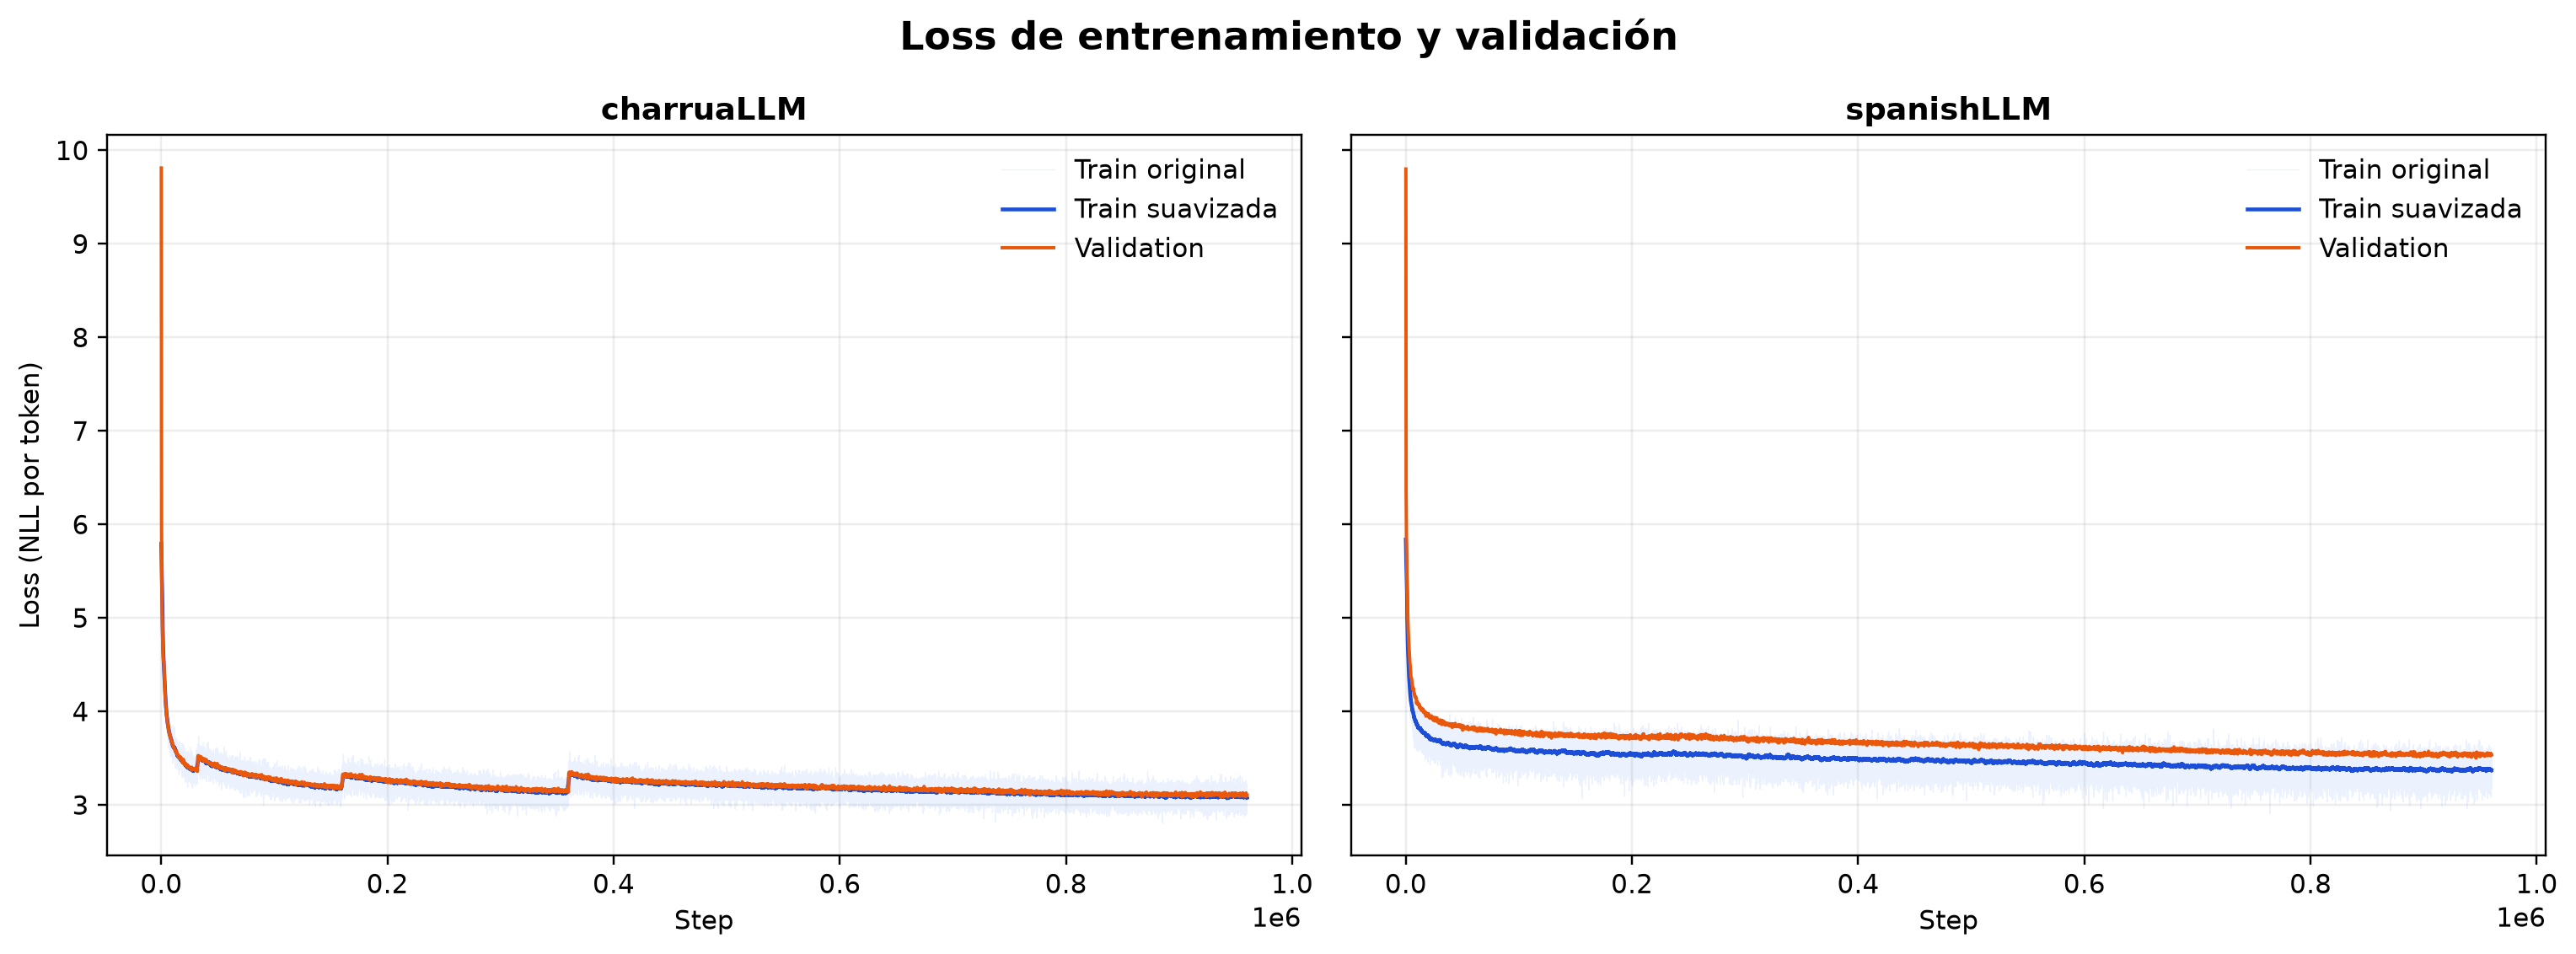
\includegraphics[width=\textwidth]{loss_modelos.png}
    \caption{Loss de entrenamiento y validación de \charrua{} y
    \spanishmodel{} hasta el paso 960.000.}
    \label{fig:loss}
\end{figure}

\begin{table}[H]
    \centering
    \caption{Resumen numérico de las curvas de validación.}
    \label{tab:loss}
    \begin{tabular}{lrrrr}
        \toprule
        Modelo & Val inicial & Mejor val & Paso del mejor & Val final \\
        \midrule
        \charrua & 9,8118 & 3,0833 & 939.250 & 3,1035 \\
        \spanishmodel & 9,8010 & 3,5004 & 946.250 & 3,5364 \\
        \bottomrule
    \end{tabular}
\end{table}

La loss de train evaluada en el paso 960.000 fue 3,0924 para \charrua{} y
3,3738 para \spanishmodel. Las dos curvas descienden fuertemente desde valores
cercanos a 9,8 y luego se estabilizan. \charrua{} alcanza una loss de
validación menor. En ambos casos la loss final es levemente superior al mínimo,
por lo que para la evaluación se utilizaron los pesos \code{best.pt}: paso
939.250 para \charrua{} y paso 946.250 para \spanishmodel.


\subsection{Resultados de exact matching}

\begin{table}[H]
    \centering
    \caption{Exact matching sobre los 834 ejemplos.}
    \label{tab:exact-global}
    \begin{tabular}{lrrr}
        \toprule
        Modelo & Aciertos & Total & Exact matching \\
        \midrule
        \charrua & 222 & 834 & 26,62\,\% \\
        \spanishmodel & 39 & 834 & 4,68\,\% \\
        \bottomrule
    \end{tabular}
\end{table}

En el conjunto completo, \charrua{} supera a \spanishmodel{} por 21,94 puntos
porcentuales y obtiene aproximadamente 5,69 veces su tasa de acierto.


\subsection{Resultados de NLL}

\begin{table}[H]
    \centering
    \small
    \caption{Resultados agregados de NLL sobre los 834 ejemplos.}
    \label{tab:nll-global}
    \begin{tabular}{lrrrr}
        \toprule
        Modelo & NLL/palabra & NLL/token & Perplexity/token & Prob. palabra \\
        \midrule
        \charrua & 4,1396 & 2,3534 & 10,52 & 25,06\,\% \\
        \spanishmodel & 22,8143 & 7,4529 & 1.724,80 & 3,00\,\% \\
        \bottomrule
    \end{tabular}
\end{table}

La cantidad total de tokens objetivo fue 1.467 para \charrua{} y 2.553 para
\spanishmodel, equivalentes a 1,76 y 3,06 tokens por palabra respectivamente.

\charrua{} asigna mucha más probabilidad a las palabras correctas y obtiene una
NLL sustancialmente menor. El resultado es consistente con exact matching, pero
la NLL aporta información adicional: permite observar si el objetivo tenía una
probabilidad razonable incluso cuando otra palabra quedó en primer lugar.

La comparación de NLL por token y perplexity requiere cautela porque cada
modelo utiliza su propio tokenizer. \spanishmodel{} divide las palabras
objetivo en muchos más tokens, en parte porque fue entrenado con texto en
minúsculas y el dataset contiene nombres propios y mayúsculas. La NLL total por
palabra compara la probabilidad asignada a la misma cadena objetivo y es una
referencia más interpretable entre los dos sistemas, pero tampoco separa por sí
sola el efecto del modelo del efecto de su tokenizer. Una evaluación futura
podría sumar bits por byte o bits por carácter para reducir esta dependencia.


\subsection{Análisis cualitativo de las predicciones}

La comparación exacta no captura por completo la calidad lingüística de las
continuaciones. Para ilustrar los comportamientos observados se seleccionaron
diez ejemplos del archivo \code{exact\_matching\_results.csv}. Cada ejemplo se
presenta con la afirmación completa, el prompt utilizado, las predicciones de
ambos modelos y el análisis cualitativo correspondiente.

\subsubsection{Alternativas semánticamente relacionadas}

\begin{enumerate}[leftmargin=*, itemsep=0.9em]
    \item \textbf{Afirmación (id 0):} ``El Pereira Rossell es un hospital.''\\
          \textbf{Prompt:} ``El Pereira Rossell es un''\\
          \textbf{Predicciones:}\\
          \hspace*{1em}\charrua{}: \code{centro}\\
          \hspace*{1em}\spanishmodel{}: \code{tipo}\\
          \textbf{Análisis cualitativo:} \code{centro} no coincide exactamente
          con el objetivo, pero es una continuación semánticamente plausible.

    \item \textbf{Afirmación (id 1):} ``El sector de alojamiento y servicios de
          comida envió la mayor cantidad de trabajadores al seguro de desempleo.''\\
          \textbf{Prompt:} ``El sector de alojamiento y servicios de comida envió
          la mayor cantidad de trabajadores al seguro de''\\
          \textbf{Predicciones:}\\
          \hspace*{1em}\charrua{}: \code{paro}\\
          \hspace*{1em}\spanishmodel{}: \code{vida}\\
          \textbf{Análisis cualitativo:} \code{paro} es una alternativa léxica
          relacionada con el dominio laboral, mientras que \code{vida} no guarda
          una relación clara con el contexto.

    \item \textbf{Afirmación (id 23):} ``Los clubes de la B y de la C recibieron
          donaciones de alimentos y productos de limpieza.''\\
          \textbf{Prompt:} ``Los clubes de la B y de la C recibieron donaciones de
          alimentos y productos de''\\
          \textbf{Predicciones:}\\
          \hspace*{1em}\charrua{}: \code{higiene}\\
          \hspace*{1em}\spanishmodel{}: \code{origen}\\
          \textbf{Análisis cualitativo:} \code{higiene} conserva el campo
          semántico de la limpieza; \code{origen} resulta irrelevante.

    \item \textbf{Afirmación (id 44):} ``Las policlínicas estuvieron cerradas
          desde que se conocieron los primeros casos de covid-19.''\\
          \textbf{Prompt:} ``Las policlínicas estuvieron cerradas desde que se
          conocieron los primeros casos de''\\
          \textbf{Predicciones:}\\
          \hspace*{1em}\charrua{}: \code{coronavirus}\\
          \hspace*{1em}\spanishmodel{}: \code{cáncer}\\
          \textbf{Análisis cualitativo:} \code{coronavirus} es otra
          denominación relacionada con el objetivo, mientras que \code{cáncer}
          cambia de enfermedad.
\end{enumerate}

Estos casos muestran que algunos errores de \charrua{} pueden ser razonables
desde el punto de vista lingüístico o semántico, aunque exact matching los
clasifique como incorrectos. También muestran una diferencia cualitativa frente
a continuaciones de \spanishmodel{} que no guardan relación clara con el contexto.

\subsubsection{Aciertos de entidades y expresiones institucionales}

\begin{enumerate}[leftmargin=*, itemsep=0.9em]
    \item \textbf{Afirmación (id 13):} ``Jair Bolsonaro fue presidente de Brasil.''\\
          \textbf{Prompt:} ``Jair Bolsonaro fue presidente de''\\
          \textbf{Predicciones:}\\
          \hspace*{1em}\charrua{}: \code{Brasil}\\
          \hspace*{1em}\spanishmodel{}: \code{la}\\
          \textbf{Análisis cualitativo:} \charrua{} completa correctamente una
          entidad geopolítica, mientras que \spanishmodel{} produce una palabra
          funcional sin completar la afirmación.

    \item \textbf{Afirmación (id 122):} ``Daniel Salinas fue ministro de Salud
          Pública.''\\
          \textbf{Prompt:} ``Daniel Salinas fue ministro de Salud''\\
          \textbf{Predicciones:}\\
          \hspace*{1em}\charrua{}: \code{Pública}\\
          \hspace*{1em}\spanishmodel{}: \code{í!}\\
          \textbf{Análisis cualitativo:} \charrua{} completa correctamente una
          expresión institucional de varias palabras.

    \item \textbf{Afirmación (id 5):} ``La OPS es la Organización Panamericana
          de la Salud.''\\
          \textbf{Prompt:} ``La OPS es la Organización Panamericana de la''\\
          \textbf{Predicciones:}\\
          \hspace*{1em}\charrua{}: \code{Salud}\\
          \hspace*{1em}\spanishmodel{}: \code{rrrr...}\\
          \textbf{Análisis cualitativo:} \charrua{} acierta, mientras que
          \spanishmodel{} produce una secuencia repetitiva marcada como truncada
          en el archivo de resultados.
\end{enumerate}

Estos aciertos sugieren que el modelo especializado puede memorizar o recuperar
con mayor facilidad nombres propios, instituciones y expresiones frecuentes en
el dominio periodístico uruguayo. La comparación no permite atribuir cada caso
exclusivamente al dominio, porque ambos modelos también tienen tokenizadores
distintos.

\subsubsection{Puntuación, capitalización y continuaciones incompletas}

\begin{enumerate}[leftmargin=*, itemsep=0.9em]
    \item \textbf{Afirmación (id 16):} ``El canciller de Brasil fue Ernesto
          Araújo.''\\
          \textbf{Prompt:} ``El canciller de Brasil fue Ernesto''\\
          \textbf{Predicciones:}\\
          \hspace*{1em}\charrua{}: \code{Araújo,}\\
          \hspace*{1em}\spanishmodel{}: \code{íta}\\
          \textbf{Análisis cualitativo:} \charrua{} recupera el nombre correcto,
          pero añade una coma y obtiene un falso negativo de exact matching.

    \item \textbf{Afirmación (id 25):} ``Se deja constancia de los datos de
          coronavirus en la página web del Sistema Nacional de Emergencias
          (SINAE).''\\
          \textbf{Prompt:} ``Se deja constancia de los datos de coronavirus en la
          página web del Sistema Nacional de Emergencias''\\
          \textbf{Predicciones:}\\
          \hspace*{1em}\charrua{}: \code{(Sinae)}\\
          \hspace*{1em}\spanishmodel{}: \code{y}\\
          \textbf{Análisis cualitativo:} el error de \charrua{} es principalmente
          de capitalización, mientras que \spanishmodel{} no recupera la sigla.

    \item \textbf{Afirmación (id 57):} ``Crea fue la principal herramienta que
          utilizaron los docentes y alumnos en la educación virtual escolar.''\\
          \textbf{Prompt:} ``Crea fue la principal herramienta que utilizaron los
          docentes y alumnos en la educación virtual''\\
          \textbf{Predicciones:}\\
          \hspace*{1em}\charrua{}: punto final, sin palabra\\
          \hspace*{1em}\spanishmodel{}: coma\\
          \textbf{Análisis cualitativo:} ambos modelos detienen la generación sin
          completar la palabra objetivo.
\end{enumerate}

Estos ejemplos muestran que la puntuación y la capitalización influyen
directamente en exact matching. También evidencian que una generación puede
detenerse antes de completar la palabra objetivo. Por ello, la métrica estricta
debe interpretarse junto con una inspección cualitativa y, cuando esté disponible,
con medidas probabilísticas como la NLL.


\subsection{Interpretación general}

Los resultados apoyan la hipótesis de que la especialización de dominio es
importante. Con la misma arquitectura y cantidad de parámetros, el modelo
entrenado con noticias uruguayas predice mejor palabras de afirmaciones basadas
en noticias uruguayas que el modelo entrenado con un corpus general en español.
Esta conclusión es consistente con ROUBERTa, que también obtuvo mejores
resultados con UY22 que con un corpus general cinco veces mayor y superó a BETO
y XLM-RoBERTa en su evaluación de palabras enmascaradas no vistas.

La diferencia puede explicarse por varios factores relacionados:

\begin{enumerate}
    \item \charrua{} fue entrenado con el dominio periodístico uruguayo.
    \item Su tokenizer representa con menos tokens las palabras evaluadas.
    \item El corpus general mezcla dominios muy heterogéneos.
    \item \spanishmodel{} fue entrenado con texto en minúsculas, mientras la
          evaluación conserva capitalización y numerosos nombres propios.
    \item Los modelos son pequeños, por lo que la selección del dominio y el
          uso del vocabulario tienen un impacto particularmente visible.
\end{enumerate}

Estos resultados no demuestran que un modelo general de español sea
intrínsecamente inferior. Muestran que, bajo esta arquitectura, estos datos y
este protocolo, el corpus especializado ofrece una ventaja clara para el
benchmark seleccionado.


\section{Conclusiones}

Se construyeron y entrenaron dos modelos Transformer decoder-only de 17,1
millones de parámetros: \charrua, especializado en noticias uruguayas, y
\spanishmodel, entrenado con un corpus general en español. Además, se creó un
nuevo dataset de completado de 834 ejemplos a partir de afirmaciones de QuUANTO
y se implementaron dos evaluaciones complementarias.

El proyecto retoma el corpus UY22 introducido junto con ROUBERTa, pero explora
una arquitectura y una tarea distintas. Mientras ROUBERTa es un encoder
bidireccional entrenado con masked language modeling, \charrua{} es un decoder
causal entrenado para generación. A pesar de esta diferencia, ambos trabajos
ofrecen evidencia convergente sobre el valor de los datos de prensa uruguaya y
la especialización de dominio.

\charrua{} obtuvo 26,62\,\% de exact matching frente a 4,68\,\% de
\spanishmodel{} sobre los 834 ejemplos combinados. También alcanzó una NLL media por palabra considerablemente menor: 4,1396
frente a 22,8143 en el conjunto completo. Las curvas de entrenamiento muestran
asimismo una mejor loss de validación para \charrua: 3,0833 frente a 3,5004.

En conjunto, el experimento muestra que un modelo pequeño puede beneficiarse
fuertemente de datos y tokenización adaptados al dominio. También evidencia que
una evaluación responsable debe complementar la predicción exacta con medidas
probabilísticas y explicitar las diferencias de tokenización, capitalización y
posible solapamiento de datos.


\section{Limitaciones y trabajo futuro}

\begin{itemize}
    \item No se realizó una búsqueda sistemática de hiperparámetros. Sería útil
          comparar distintas tasas de aprendizaje, tamaños de modelo, longitudes
          de contexto y regímenes de entrenamiento.
    \item Sería conveniente analizar cualitativamente una muestra amplia de
          errores y agruparlos, por ejemplo, en sinónimos, nombres propios,
          errores morfológicos, errores sintácticos y falta de conocimiento.
    \item Sería útil entrenar con el dataset convertido a minúsculas para
          coincidir con el otro modelo.
    \item También podría reportarse una métrica auxiliar que considere
          equivalentes las predicciones que solo difieren en mayúsculas y
          minúsculas. La métrica principal debería mantenerse sensible a la
          capitalización para conservar la evaluación original.
\end{itemize}


\section{Archivos producidos}

\begin{itemize}
    \item \code{final\_dataset.csv}: dataset de 834 ejemplos.
    \item \code{exact\_matching\_results.csv}: predicciones y exact matching.
    \item \code{nll\_results.csv}: NLL y probabilidades por palabra y token.
    \item \code{charruaLLM/best.pt}: mejor checkpoint de \charrua.
    \item \code{spanishLLM/best.pt}: mejor checkpoint de \spanishmodel.
    \item \code{charruaLLM/losses.csv}: historial de entrenamiento.
    \item \code{spanishLLM/losses.csv}: historial de entrenamiento.
    \item \code{notebook.ipynb}: preparación, evaluación y visualización.
\end{itemize}


\clearpage
\begin{thebibliography}{99}

\bibitem{filevich2024}
Filevich, J. P., Marco, G., Castro, S., Chiruzzo, L. y Rosá, A. (2024).
\newblock \emph{A Language Model Trained on Uruguayan Spanish News Text}.
\newblock Proceedings of the Second International Workshop Towards Digital
Language Equality (TDLE), LREC-COLING 2024, pp. 53--60.
\newblock \url{https://aclanthology.org/2024.tdle-1.5.pdf}

\bibitem{hoffmann2022}
Hoffmann, J. et al. (2022).
\newblock \emph{Training Compute-Optimal Large Language Models}.
\newblock arXiv:2203.15556.
\newblock \url{https://arxiv.org/abs/2203.15556}

\bibitem{liu2019}
Liu, Y. et al. (2019).
\newblock \emph{RoBERTa: A Robustly Optimized BERT Pretraining Approach}.
\newblock arXiv:1907.11692.
\newblock \url{https://arxiv.org/abs/1907.11692}

\bibitem{radford2019}
Radford, A., Wu, J., Child, R., Luan, D., Amodei, D. y Sutskever, I. (2019).
\newblock \emph{Language Models are Unsupervised Multitask Learners}.
\newblock \url{https://cdn.openai.com/better-language-models/language-models.pdf}

\bibitem{rosa2022}
Rosá, A., Chiruzzo, L., Bouza, L. et al. (2022).
\newblock \emph{Overview of QuALES at IberLEF 2022: Question Answering
Learning from Examples in Spanish}.
\newblock \url{https://rua.ua.es/dspace/handle/10045/127433}

\bibitem{quanto}
QuUANTO.
\newblock \emph{QuALES-derived Uruguay Assertions for Neural Training Objectives}.
\newblock Repositorio del dataset.
\newblock \url{https://github.com/McBruno712/QuUANTO}

\bibitem{sennrich2016}
Sennrich, R., Haddow, B. y Birch, A. (2016).
\newblock \emph{Neural Machine Translation of Rare Words with Subword Units}.
\newblock Proceedings of ACL 2016, pp. 1715--1725.
\newblock \url{https://aclanthology.org/P16-1162/}

\bibitem{vaswani2017}
Vaswani, A. et al. (2017).
\newblock \emph{Attention Is All You Need}.
\newblock arXiv:1706.03762.
\newblock \url{https://arxiv.org/abs/1706.03762}

\bibitem{canete}
Cañete, J.
\newblock \emph{Large Spanish Corpus}.
\newblock Hugging Face Datasets.
\newblock \url{https://huggingface.co/datasets/josecannete/large_spanish_corpus}

\bibitem{opus}
OPUS.
\newblock \emph{Open Parallel Corpus}.
\newblock \url{https://opus.nlpl.eu/}

\end{thebibliography}

\end{document}
